\documentclass[11pt]{article}


\usepackage[letterpaper,margin=1in]{geometry}
\usepackage{graphicx}
\usepackage{hyperref}
\usepackage{amsmath}
\usepackage{amssymb}
\usepackage{bm}
\usepackage{listings}
\usepackage{color}
\usepackage{tikz}
\usepackage{hologo}% or use package holog

\usepackage{empheq}
\usepackage{color}

\usetikzlibrary{decorations.pathmorphing,patterns}

\definecolor{myblue}{rgb}{.92549, .98824, 0.95686}
\newlength\mytemplen
\newsavebox\mytempbox

\makeatletter
\newcommand\mybluebox{%
    \@ifnextchar[%]
       {\@mybluebox}%
       {\@mybluebox[0pt]}}

\def\@mybluebox[#1]{%
    \@ifnextchar[%]
       {\@@mybluebox[#1]}%
       {\@@mybluebox[#1][0pt]}}

\def\@@mybluebox[#1][#2]#3{
    \sbox\mytempbox{#3}%
    \mytemplen\ht\mytempbox
    \advance\mytemplen #1\relax
    \ht\mytempbox\mytemplen
    \mytemplen\dp\mytempbox
    \advance\mytemplen #2\relax
    \dp\mytempbox\mytemplen
    \colorbox{myblue}{\hspace{1em}\usebox{\mytempbox}\hspace{1em}}}

\makeatother

\definecolor{dkgreen}{rgb}{0,0.6,0}
\definecolor{gray}{rgb}{0.5,0.5,0.5}
\definecolor{mauve}{rgb}{0.58,0,0.82}

\lstset{frame=tb,
  language=Python,
  aboveskip=3mm,
  belowskip=3mm,
  showstringspaces=false,
  columns=flexible,
  basicstyle={\small\ttfamily},
  numbers=none,
  numberstyle=\tiny\color{gray},
  keywordstyle=\color{blue},
  commentstyle=\color{dkgreen},
  stringstyle=\color{mauve},
  breaklines=true,
  breakatwhitespace=true,
  tabsize=3
}

\graphicspath{ {./images/} }

\def\changemargin#1#2{\list{}{\rightmargin#2\leftmargin#1}\item[]}
\let\endchangemargin=\endlist 

% define info for title page
\title{AMATH 271 Final Project: \\ Brachistochrone}
\author{Omer Sipra, Kamalesh Reddy}
\date{\today}

\newcommand{\Lagr}{\mathcal{L}}

\begin{document}

% make the title page
\maketitle

% use enumerate to make a numbered list; in this case, a list of problem solutions

\begin{enumerate}

\item Example diagrams:

\begin{center}
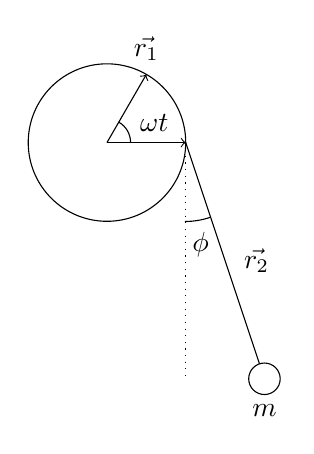
\begin{tikzpicture}
  \draw (0, 0) circle (1cm);
  \draw (1, 0) -- (2, -3);
  \draw [dotted] (1, 0) -- (1, -3);
  \draw (1.316, -0.948) arc (-71:-90:1);
  \node at (1.19, -1.3) {$\phi$};
  \node at (1.9, -1.5) {$\vec{r_2}$};
  \draw [fill=white] (2, -3) circle (0.2cm);
  \node at (2, -3.4) {$m$};
  \draw [->] (0, 0) -- (1, 0);
  \draw [->] (0, 0) -- (0.5, 1.73/2);
  \draw (0.3, 0) arc (0:60:0.3);
  \node at (0.5, 1.19) {$\vec{r_1}$};
  \node at (0.6, 0.25) {$\omega t$};

\end{tikzpicture}
\end{center}

\begin{center}
  \begin{tikzpicture}
    \draw [dotted] (1, 2) -- (1, -3);
    \draw [dotted] (-1, 2) -- (-1, -3);
    \draw [fill = white] (0, 0) rectangle (2, 1);
    \draw (0.5, -0.2) circle (0.2cm);
    \draw (1.5, -0.2) circle (0.2cm); 
    \draw [->] (-1, 2) -- (1, 2);
    \draw [<-] (1.316, -0.948) arc (-71:-90:1);
    \node at (1.19, -1.3) {$\phi$};
    \node at (1.9, -1.5) {$\vec{r_2}$};
    \draw (1, 0) -- (2, -3);
    \draw [fill=white] (2, -3) circle (0.2cm);
    \draw [decoration={aspect=0.3, segment length=3mm, amplitude=3mm,coil},decorate] (-4, 0.5) -- (-1, 0.5);
    \draw (-1, 0.5) -- (0, 0.5);
    \draw (-5, 0.5) -- (-4, 0.5);
    \draw (-5, -0.4) -- (3, -0.4); 
    \draw (-5, -0.4) -- (-5, 3); 
    \node at (-2.65, 1.2) {$k$};
    \node at (1, 0.5) {$m$};
    \node at (1.95, -3.5) {$M$};
    \node at (0, 2.3) {$\vec{r_1}$};
    \draw [->] (-7, -0.4) -- (-6, -0.4);
    \draw [->] (-7, -0.4) -- (-7, -1.4);
    \node at (-5.8, -0.4) {$x$};
    \node at (-7, -1.65) {$y$};
  \end{tikzpicture}
  \end{center}

Example Python code:
\begin{lstlisting}
  # Prints example twice
  for i in [0, 1]:
    print("example")
  #
  #
  #
\end{lstlisting}

So, using Python, we solve:
\begin{center}
  $\dfrac{d}{dt}$
$\begin{bmatrix}
  x \\
  \phi \\
  \dot{x} \\
  \dot{\phi} 
\end{bmatrix}$
$ = $
$\begin{bmatrix}
  \dot{x} \\
  \dot{\phi} \\
  \cfrac{ML\dot{\phi}\sin(\phi) - kx + Mg\sin(\phi)\cos(\phi)}{(m+M) - M\cos^2(\phi)} \\
  \cfrac{M^2L\dot{\phi}^2\cos(\phi)\sin(\phi) - Mkx\cos(\phi) + (m+M)Mg\sin(\phi)}{M^2 L \cos^2(\phi) - (m+M)ML}
\end{bmatrix}$
\end{center}

Where $m = 1, M = 1, L = 1, g = 1,$ and $k = 2$ are the given parameters.

\end{enumerate}

\end{document}